\usepackage[authoryear,round]{natbib}
\usepackage{multirow}

\newcommand{\sheetnum}{%
	08
}
%\setcounter{section}{\sheetnum-3}
\newcommand{\tutorialtitle}{%
    K-means Clustering and Pairwise Clustering
}
\newcommand{\tutorialtitleshort}{%
	Clustering
}
% for slides
\subtitle{\sheetnum \tutorialtitle}

%\maxdeadcycles=1000 % Workaround for ! Output loop---100 consecutive dead cycles because of too many figures

% The following use of algroithms does not work well with the notes:
%
%
%
%
% instead use the following for your algorithms:
%
%\begin{figure}[!t]
%\removelatexerror
%\begin{algorithm}[H]
    % your algo here
    %\label{alg:algolabel}
    %\caption{algocaption}
%\end{algorithm}
%\end{figure}
%\begin{algorithm}
% Below is the definition for the command \removelatexerror:
\makeatletter
\newcommand{\removelatexerror}{\let\@latex@error\@gobble}
\makeatother

\begin{document} %%%%%%%%%%%%%%%%%%%%%%%%%%%%%%%%%%%%%%%%%%%%%%%%%%%%%%%

\sheet{\sheetnum}{\tutorialtitleshort}

\ttopic{\tutorialtitle}

\columnratio{0.2,0.8}\textbf{}
\begin{paracol}{2}
%\setlength{\columnseprule}{0.1pt}
%\setlength{\columnsep}{5em}

\begin{rightcolumn}

% notes version will ignore it
\begin{frame}
\titlepage
\end{frame}

\begin{frame}
\tableofcontents
\end{frame}

\newpage

\mode<all>


\begin{frame}
\underline{Outline}
\begin{itemize}
\item K-means clustering
    \begin{itemize}
    \item the batch algorithm
    \item the online algorithm
    \item mini-batch learning
    \item the soft clustering algorithm
    \end{itemize}
\item pairwise clustering
\end{itemize}
\end{frame}

\begin{frame}
\section{K-means}

\underline{In plain English:}\\

Data is observed. We want to be able to describe some ``structure'' in the data.
We base our approach on something very simple and intuitive: 
A set of 
objects (points) that share common features tend to fall in some region. A second set of objects that also share common features but which are different from the first set fall in another region.
This ``structure'' we are describing groups, ``clusters'' a collection of points based on their proximity to a region.  
A point that is further away from this collection and closer to another is grouped with the points associated with that other region. 
We do have to decide on how many clusters we think exist in a dataset.

\question{What does clustering give us?}
 
- Eventually, instead of describing each point by its absolute location, we will be able to describe it by the cluster it is assigned to. 
We will also be able to describe the entire dataset by the partitions we've found that separate the clusters.

\end{frame}
\begin{frame}

\underline{Problem:}\\

Group the dataset $\left\{ \vec x^{(1)}, \vec x^{(2)}, \ldots, \vec x^{(p)} \right\}$, where $\vec x \in \R^N$, into $M$ clusters\footnote{$M$ is actually equivalent to the $K$ in $K$-means.}.

\underline{The K-means approach:}\\

Determine $M$ ``good'' prototypes $\vec w_1, \ldots, \vec w_M \in R^N$ and assign each data point $\vec x^{(\alpha)}$ to the prototype closest to it.\\

TODO: image

The assignment is formalized by introducing the following assignment variable $m_q^{(\alpha)}$ for each point $\alpha$ and each cluster $q$:

\begin{equation}
\label{eq:assignment}
	m_q^{(\alpha)} := \left\{ \begin{array}{ll}
		1, & \text{if } \vec{x}^{(\alpha)} \text{ belongs to cluster } q
		\\\\
		0, & \text{else}
	\end{array} \right. 
\end{equation}

$q$ is used as the cluster index. We have a total of $p \cdot M$ assignment variables for a dataset with $p$ points and choice of number of clusters $M$.

$m_q^{(\alpha)}$ is a binary variable and with the normalization:

\begin{equation}
    \label{eq:assignmentnormalization}
	\sum\limits_q m_q^{(\alpha)} = 1,
\end{equation}
we limit the assignment of each point to only one cluster. We refer to this as a ``hard'' assignment\footnote{This will be relaxed when we talk about ``soft'' K-means.}.

A solution to our problem is one that finds finds the location of the prototypes $\vec w_q$ and assigns all points that are optimal in terms of the following cost which measures the average distance between a prototype and the subset of points assigned to it:

\begin{align}
\label{eq:kmeanscost}
E_{ \big[ \big\{ m_q^{(\alpha)} \big\}, \big\{ \vec{w}_q \big\} 
		\big] }^T &= \frac{1}{p} \sum\limits_{q,\alpha} m_q^{(\alpha)}
		\big( \vec{x}^{(\alpha)} - \vec{w}_q \big)^2\\
        &= \frac{1}{p} \sum_{\alpha=1}^{p} \sum_{q=1}^{M} m_q^{(\alpha)}
		\big( \vec{x}^{(\alpha)} - \vec{w}_q \big)^2 \eqexcl \underset{\big\{ m_q^{(\alpha)} \big\}, \big\{ \vec{w}_q \big\}}{\min}
\end{align}

\notesonly{
When we consider the definition of $m_q^{(\alpha)}$ as \emph{binary variables} as provided by \eqref{eq:assignment} and their normalization as in \eqref{eq:assignmentnormalization}, we realize that for each point $\alpha$ only one of its $m_q^{(\alpha)}$ is non-zero (and =1). Therefore, we are effectively evaluating the distance $\big( \vec{x}^{(\alpha)} - \vec{w}_q \big)^2$ only \textbf{once} for that point $\alpha$, namely it's distance only to the one cluster $q$ that point is assigned to.

This simplifies our expression for the cost function:


}
\begin{align}
\label{eq:kmeanscostsimple}
E_{ \big[ \big\{ m_q^{(\alpha)} \big\}, \big\{ \vec{w}_q \big\} 
		\big] }^T 
        &= \frac{1}{p} \sum_{\alpha=1}^{p}
		\big( \vec{x}^{(\alpha)} - \vec{w}_q \big)^2 \eqexcl \underset{\big\{ m_q^{(\alpha)} \big\}, \big\{ \vec{w}_q \big\}}{\min}
\end{align}


\notesonly
{
Where the cost is minimized over the set of discrete variables $\big\{ m_q^{(\alpha)} \big\}$ as well as the set of continuous variables $\big\{ \vec{w}_q \big\}$.

Minimizing the average distance between each prototype $\vec w_q$ and the points assigned to it leads to partitioning the data into $M$ clusters such that a point is assigned to a cluster $q$ because it is closest to $\vec w_q$.
}
\end{frame}

\begin{frame}
\section{Batch K-means: Algorithm overview}

\notesonly{
The way we've approached previous optimization problems is to derive how the parameters are updated to minimize the cost function and then we look at the algorithm that make use of the derived update rules to find a solution to the problem. Given the simplicity of the K-means algorithm, we will opt to first look at the algorihtm that implements K-means to understand how it operates and interesting aspects of the solution that it finds. We will then follow this by discussing the derivations we encountered in the algorithm (e.g. the update rule)

\underline{How does K-means work?} 
}

An iterative two-step procedure after initializing $\big\{ \vec{w}_q \big\}$:
\begin{enumerate}
\item \textbf{assign} each point to its \emph{nearest} prtototype (nearest $\corresponds$ smallest Euclidiean distance.)
\item \textbf{update} all cluster prototypes by moving them their cluster's center of mass.
\end{enumerate}



\end{frame}

\begin{frame}
\section{Batch K-means: Algorithm details}

\vspace{-0.4cm}
\begin{figure}[!th]
\footnotesize
\removelatexerror
\begin{algorithm}[H]
\DontPrintSemicolon
  random initialization of prototypes, e.g.\ $\vec{w}_{q} = \langle \vec{x} \rangle +\vec{\eta}_{q}, \hspace{0.2cm} \vec{\eta}_{q}  \text{ small random vector}$\;
  \Begin(loop){
  (1) choose  $m_q^{(\alpha)}$ such that $E^T$ is minimal for the given prototypes\;
\[ m_q^{(\alpha)} = \left\{ \begin{array}{ll}
	1, & \text{if } q = \argmin_{\gamma} \big| \vec{x}^{(\alpha)}
		- \vec{w}_{\gamma} \big| \\
	0, & \text{else}
\end{array} \right. \]
$\Rightarrow$ assign \textbf{every} data point to its nearest prototype \;
\;
(2) choose  $\vec{w}_q$ such that $E^T$ is minimal for the \textbf{new} assignments\;
\[ \vec{w}_q = \frac{\sum\limits_{\alpha} m_q^{(\alpha)} \vec{x}^{(\alpha)}}{
	\sum\limits_{\alpha} m_q^{(\alpha)}}
\]
$\Rightarrow$ set $\vec{w}_q$ to the center of mass of its assigned data
}
    \label{alg:batch-k-means}
    \caption{batch K-means}
\end{algorithm}
\end{figure}
\end{frame}

The steps for finding the optimal prototype locations and assignments are described in Algorithm \ref{alg:batch-k-means}.
It is important to understand that a single iteration, takes \textbf{all} points into account. This is not a loop that iterates over the individual points. Each iteration deals with assignment of \textbf{all} points and updating the location of the prototypes considering all data points collectively within that iteration.
The stopping criterion for the batch K-means algorithm\ref{alg:batch-k-means}, i.e. when to stop the loop, can be chosen by detecing that the location of prototypes are no longer moving. Alternatively, one could keep track of the difference in the value of $E^T$ between two successive iterations until it reaches some desired threshold.
 
Things to note about \emph{batch K-means}:

\begin{enumerate}
\item $E^T$ is \emph{non-increasing}\footnote{Non-increasing $\corresponds$ decreasing OR unchanged.}. We either move to an improved solution with lower cost or the cost remains unchanged.
\item This is a nonconvex optimization problem. This means that we may arrive at local optima which yield bad solutions. Additionally, the global minimum is not unique. There exist $M! = \prod_{i=1}^{M} i$ different assignments with the same lowest cost. This is a result of permutation symmetry. If we suddenly start labeling all points assigned to cluster $4 \rightarrow 7$, and simultaneously label all points originally assigned to $7 \rightarrow 4$, the cost remains unchanged. 
The algorithm is indifferent to the index value of a cluster. The cluster indices are simply ``names'' to differntiate between the clusters and changing their names does not alter the solution obtained.
 
\end{enumerate}

\begin{frame}

\question{How are is K-means an optimziation algorithm?}

\slidesonly{
Show how updating the protptypes by $\vec{w}_q = \frac{\sum\limits_{\alpha} m_q^{(\alpha)}
		\vec{x}^{(\alpha)}}{\sum\limits_{\alpha} m_q^{(\alpha)}}$ minimizes $E^T$.
}

\end{frame}

We've seen how one would implement K-means. More specifically, we've seen that the prototypes $\vec w_q$ are updated every iteration such that they represent the mean of the points assigned to them in that iteration. However, we have yet to show that this iterative method effecitvley minimizes $E^T$. We do so by evaluating the gradient, finding the zero-crossing. We are effectively looking for the extrema of the cost function $E^T$.

Recall the definition for the cost function:

\begin{frame}
\begin{equation}
E_{ \big[ \big\{ m_q^{(\alpha)} \big\}, \big\{ \vec{w}_q \big\} 
		\big] }^T = \frac{1}{p} \sum\limits_{q,\alpha} m_q^{(\alpha)}
		\big( \vec{x}^{(\alpha)} - \vec{w}_q \big)^2 \eqexcl \min
\end{equation}

The condition for an extremum is as follows:
\begin{align}
	\frac{\partial}{\partial \vec{w}_q} E^T
	&=
	\frac{\partial}{\partial \vec{w}_q} \bigg\{ \frac{1}{p} 
	\sum\limits_{q', \, \alpha} m_{q^{'}}^{(\alpha)} 
	\big( \vec{x}^{(\alpha)} - \vec{w}_{q^{'}} \big)^2 \bigg\} \\
	& = -\frac{2}{p} \sum\limits_{\alpha} m_q^{(\alpha)} 
		\big( \vec{x}^{(\alpha)} - \vec{w}_q \big) \eqexcl 0
\end{align}
\slidesonly{

Solve for $\vec w_q$...
}

\end{frame}
\begin{frame}

Solve for $\vec w_q$:


\begin{align}
 -\frac{2}{p} \sum\limits_{\alpha} m_q^{(\alpha)} 
		\big( \vec{x}^{(\alpha)} - \vec{w}_q \big) &= 0 \quad (\text{\small omit the constant}\; -2/p),\\
 \sum\limits_{\alpha} m_q^{(\alpha)} 
		\big( \vec{x}^{(\alpha)} - \vec{w}_q \big) &= 0\\
 \sum\limits_{\alpha} m_q^{(\alpha)} 
		\vec{x}^{(\alpha)} &= \sum\limits_{\alpha} m_q^{(\alpha)} \vec{w}_q \\
		\vec w_q \;\text{\small does not depend on}\; &\alpha, \;\text{\small use it as a normalization factor},\\
	\leadsto \vec{w}_q &= \frac{\sum\limits_{\alpha} m_q^{(\alpha)}
		\vec{x}^{(\alpha)}}{\sum\limits_{\alpha} m_q^{(\alpha)}}
\end{align}

\end{frame}
\begin{frame}

\slidesonly{
$$
	\leadsto \vec{w}_q = \frac{\sum\limits_{\alpha} m_q^{(\alpha)}
		\vec{x}^{(\alpha)}}{\sum\limits_{\alpha} m_q^{(\alpha)}}
$$
}
Now we've found the extremum. We still need to identify if this corresponds to a maximum or minimum:


The condition for a minimum is that the second-order partial derivatives, the \emph{Hessian}, is positive:

\begin{align}
	\frac{\partial^2}{\partial \mathrm{w}_{qi} \partial \mathrm{w}_{
			q'j}} \big\{ E^T\big\}
	&=
		\frac{\partial^2}{\partial \mathrm{w}_{qi} \partial \mathrm{w}_{
			q'j}} \bigg\{ \frac{1}{p} \sum\limits_{q^{''}, \alpha}
			m_{q^{''}}^{(\alpha)} \big( \vec{x}^{(\alpha)} - \vec{w}_{q^{''}}
			\big)^2 \bigg\} \\
		& = \frac{\partial}{\partial \mathrm{w}_{q^{'}j}} \bigg\{
			-\frac{2}{p} \sum\limits_{\alpha} m_q^{(\alpha)} 
			\big( \mathrm{x}_i^{(\alpha)} - (\vec{w})_{qi}
			\big) \bigg\} \\
\notesonly{
		& = \left( \frac{2}{p} \sum\limits_{\alpha} m_q^{(\alpha)} \right)
			\delta_{ij} \delta_{qq^{'}}
			}
\end{align}
\end{frame}

\begin{frame}
\slidesonly{
\begin{align}
	\frac{\partial^2}{\partial \mathrm{w}_{qi} \partial \mathrm{w}_{
			q'j}} \big\{ E^T\big\}
	&=
		\frac{\partial^2}{\partial \mathrm{w}_{qi} \partial \mathrm{w}_{
			q'j}} \bigg\{ \frac{1}{p} \sum\limits_{q^{''}, \alpha}
			m_{q^{''}}^{(\alpha)} \big( \vec{x}^{(\alpha)} - \vec{w}_{q^{''}}
			\big)^2 \bigg\} \\
		& = \left( \frac{2}{p} \sum\limits_{\alpha} m_q^{(\alpha)} \right)
			\delta_{ij} \delta_{qq^{'}}
\end{align}
}

where $\delta_{ij}$ and $\delta_{qq^{'}}$ are the dirac-delta functions ($\delta_{ij}=1$ iff $i=j$ and $=0$ otherwise). 
Since $\frac{2}{p} \sum\limits_{\alpha} m_q^{(\alpha)}$ is always positive \notesonly{(c.f. \eqref{eq:assignmentnormalization})}:

\begin{itemize}
	 \itR The Hessian is a diagonal matrix with all positive entries $\,\to\,$ condition for minimum is always satisfied.
	 \itR however: minimizing $E^{T}$ is not a convex optimization problem (because of the combination of steps 1 and 2).
\end{itemize} 

\end{frame}

% --------------------------------------------------------------------------
\begin{frame} \frametitle{Intepreting the solution}
\begin{figure}[h]
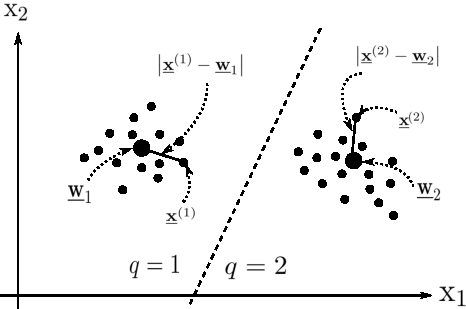
\includegraphics[width=5.0cm]{img/section4_fig2_withincluster}
\end{figure}
$$
	E_{ \big[ \big\{ m_q^{(\alpha)} \big\}, \big\{ \vec{w}_q \big\} 
		\big] }^T = \frac{1}{p} \sum\limits_{q,\alpha} m_q^{(\alpha)}
		\big( \vec{x}^{(\alpha)} - \vec{w}_q \big)^2
$$
\begin{itemize}
 \itR If $\vec{w}_q$ is center of mass $\implies$ $E^T = \mathrm{variance}$.
 \itR $E^T$ is non-increasing in every step and $E^T$ is bounded from below $\,\to\,$ K-means clustering converges to a (local) optimum of $E^T$. 
\itR $E^T$ at the solution can be interpreted as the ``size'' (variance) of the clusters.
\end{itemize} 
\end{frame}

\begin{frame}
\section{On-line K-means}

We now look at a variant of K-means that partitions the data in an \emph{online} fashion. This allows the clustering to:

\begin{figure}[!th]
\footnotesize
\removelatexerror
\begin{algorithm}[H]
  \DontPrintSemicolon
   random initialization of prototypes, e.g.\ $\vec{w}_{q} = \langle  \vec{x} \rangle +\vec{\eta}_{q},\hspace{0.2cm} \vec{\eta}_{q}  \text{ small random vector}$\;
  select learning step:   $0 < \varepsilon  \ll 1$\;
  \Begin(loop){
    choose a data point $\vec{x}^{(\alpha)}$ \;
    assign data point to its closest prototype $q$\;
    \[ q = \argmin_{\gamma} \big| \vec{x}^{(\alpha)} - \vec{w}_{\gamma} \big| \]
    change corresponding prototype according to\;
    \[ \Delta \vec{w}_q = \varepsilon \big( \vec{x}^{(\alpha)} - \vec{w}_{q} \big) \]
    change $\varepsilon$ \;
  }
  \label{alg:on-line-k-means}
  \caption{On-line K-Means}
\end{algorithm}
\end{figure}

\end{frame}
% --------------------------------------------------------------------------

% --------------------------------------------------------------------------
\begin{frame}
\frametitle{Further differences between batch and online K-means:}

Online K-means...
\begin{enumerate}
\item adapts to non-stationary data (streaming data)
\slidesonly{
\item less memory
\item faster
\begin{itemize}
    \item Step 1 updates assignment for a single point instead of all 
    \item Step 2 no longer iterates through all points
\end{itemize}
}
\notesonly{
\item mitigates the memory footprint of the algorithm by avoiding having to keep the entire dataset in memory
\item mitigates the time complexity of the algorithm in that  
    \begin{itemize}
    \item we no longer have to update the assignments of all data points (step 1) and that 
    \item updating the prototypes no longer requires iterating through all points (step 2).
    \end{itemize}
    }
\slidesonly{
\item ``Noisiness''of online K-means allows it to escape local minima.

}
 \notesonly{
\item Online K-means is more robust than batch-learning w.r.t convergence to local minima:
\begin{itemize} 
\item The noisy nature of online K-means gives it a better chance at ``escaping'' local minima. 
\item In batch K-means, $E^T$ either decreases or remains unchanged. Therefore, batch K-means from a local minimum.
\end{itemize}
}
\notesonly{
\item The quality of the solution found by online K-means depends on choosing an appropriate schedule for $\varepsilon$: Robbins-Monro conditions
}
\slidesonly{
\item Choose learning rate schedule for $\varepsilon$: Robbins-Monro conditions
}
\notesonly{(c.f. Fig \ref{fig:annealingScheduleKMeans2})}
\begin{figure}[h!]
  \centering
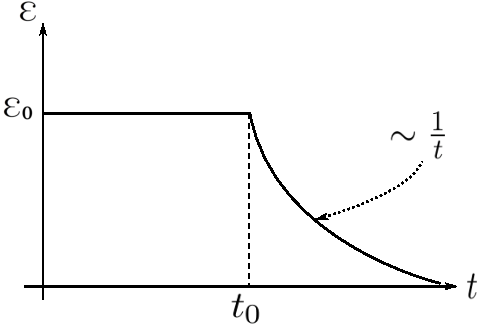
\includegraphics[height=3cm]{img/section4_fig4} 
  \caption{Decaying learning rate schedule to satisfy Robbins-Monro conditions.}
  \label{fig:annealingScheduleKMeans2}
\end{figure}
\end{enumerate}

A compromise between batch and online K-means is \emph{mini-batch K-means}.
One would modify online K-means to operate on a small subset/mini-batch of the data at a time.

\end{frame}

\begin{frame}
\section{Pairwise clustering}

\textbf{Recall} that K-means clusters points based on their proximity to some prototype.\\

\notesonly{
Another approach to describing a similar ``structure'' in the data
can be based on the following:}
\slidesonly{
\begin{figure}[h!]
  \centering
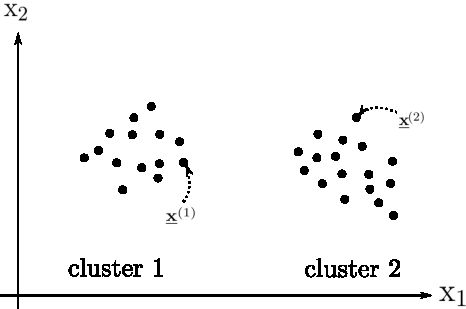
\includegraphics[height=3cm]{img/clustering} 
\end{figure}
But also:\\
}
Points that are ``close'' to one another have more in common than points that are far away from one another. 
\notesonly{
We clusters points based on their \emph{proximity to one another}. 
A point that is further away from this collection is grouped with other points that are closer to it. Pairwise clustering is about grouping points based on their pairwise relations. \
}
We will first discuss clustering based on \emph{pairwise distances} and then extend this to \emph{soft clustering}.

\end{frame}

\begin{frame}
\section{Pairwise Clustering: The data}

\notesonly{
Each data point $\vec x^{(\alpha)}$ with $\alpha = 1, \ldots, p$ is represented through its relation to all other points in the dataset by measuring pairwise distances.
}

Let $d_{\alpha \alpha^{'}}$ be the pairwise distance between any two points $\vec x^{(\alpha)}$ and $\vec x^{(\alpha')}$. Computing all pairwise distances yields the \emph{distance matrix} $\big\{ d_{\alpha \alpha^{'}} \big\}$:

\begin{equation}
\label{eq:pairwisedistdef}
d: \mathbb{R}^N \times \mathbb{R}^N 
    \rightarrow \mathbb{R}_0^+ \quad\text{ i.e.}\;\; d \ge 0
\end{equation}

The components of the distance matrix are subject to the following constraints:
\begin{itemize}
\item The distance of a point to itself is zero.
\item The distance matrix is symmetric.
\end{itemize}

\end{frame}
\begin{frame}\frametitle{Choice of distance measure}

A simple and common choice of measure is squared Euclidean distance:

\begin{equation}
\label{eq:pairwisedisteuclidean}
d_{\alpha \alpha^{'}} := \frac{1}{2} \big(
    \vec{x}^{(\alpha)} - \vec{x}^{(\alpha^{'})} \big)^2
\end{equation}

\notesonly{
Another possiblility for populating the components of the distance matrix is to base this high-dimensional relation of one point to another on \emph{scalar product}, the ``kernel trick''\footnote{As encountered in Kernel-PCA}. 
The distance is measured for a pair of points in some high-dimensional space $\phi$
}
\slidesonly{
Or elements derived via a ``kernel trick'':
}

$$
          \vec{\phi}: \vec{x}^{(\alpha)} \rightarrow
          \vec{\phi}_{\big( \vec{x}^{(\alpha)} \big)}
          \equiv \vec{\phi}^{(\alpha)}
$$

\begin{align}
			d_{\alpha \alpha^{'}} 
			& = \frac{1}{2} \big( \vec{\phi}^{(\alpha)} 
				- \vec{\phi}^{(\alpha^{'})} \big)^2 \\
			& = \frac{1}{2} \Big\{ \big( \vec{\phi}^{(\alpha)}
				\big)^2 - 2\big( \vec{\phi}^{(\alpha)} \big)^\top
				\vec{\phi}^{(\alpha^{'})} + \big(
				\vec{\phi}^{(\alpha^{'})} \big)^2 \Big\} \\
			& = \frac{1}{2} \bigg\{ k_{\big( \vec{x}^{(\alpha)},
				\vec{x}^{(\alpha)} \big)} 
				- 2k_{\big(\vec{x}^{(\alpha)},
				\vec{x}^{(\alpha^{'})} \big)}
				+ k_{\big(\vec{x}^{(\alpha^{'})},
				\vec{x}^{(\alpha^{'})} \big)}
				\bigg\}
\end{align}

\end{frame}

\begin{frame}
\slidesonly{\frametitle{Other sources for pairwise distances}}

A further alternative is to not measure pairwise distance explicitly. The data can be represented in a pairwise fashion as a result of an algroithm. Example: Sequence alignment proceducres and graph-similarity mmeasures produce pairwise representations.\\

We will rely on the \emph{squared Eucldiean distance} for our pairwise clustering algorithm.

\end{frame}

\begin{frame}
\frametitle{Pairwise Clustering: Problem statement}

\begin{itemize}
\itr set of clusters (partitions): $q = 1, \ldots, M$
\itr observations (feature vectors): $\vec{x}^{(\alpha)}, \; 
\alpha = 1, \ldots, p; \; \vec{x}^{(\alpha)} = \mathbb{R}^N$
\itr binary assignment variable:
$$ m_q^{(\alpha)} := \left\{ \begin{array}{ll}
		1, & \text{if object } \alpha \text{ belongs to cluster } q \\\\
		0, & \text{otherwise}
	\end{array} \right.
$$
\itr distance matrix $d_{\alpha \alpha^{'}}$ populated using squared Euclidean distance:
$$
	d_{\alpha \alpha^{'}} := \frac{1}{2} \big( \vec{x}^{(\alpha)} 
		- \vec{x}^{(\alpha^{'})} \big)^2
$$
\end{itemize}
\end{frame}
\begin{frame}
\frametitle{Cost function \& model selection}
\begin{align}
E_{ \big[ \big\{ m_q^{(\alpha)} \big\} \big] }
	&= \frac{1}{2p} \sum\limits_q \sum\limits_{\alpha}
	 \overbrace{ \frac{\sum\limits_{\alpha^{'}} 
		m_q^{(\alpha)}m_q^{(\alpha^{'})} d_{\alpha \alpha^{'}}}{
                \sum\limits_{\alpha'} m_q^{(\alpha')}
		}}^{ \substack{	\text{avg. distance between} \\
				\alpha \text{ and \textbf{all other} objects $\alpha'$} \\
				\text{from the \textbf{same} cluster } q}}\\
&= \frac{1}{2p} \sum\limits_q \frac{ \sum\limits_{\alpha \alpha^{'}}
		m_q^{(\alpha)} m_q^{(\alpha^{'})} \big( \vec{x}^{(\alpha)}
		-\vec{x}^{(\alpha^{'})} \big)^2 }{
			\sum\limits_{\alpha} m_q^{(\alpha)}}
	\eqexcl \min
\end{align}
            
\end{frame}

\begin{frame}\frametitle{Relation of pairwise clustering to K-means}

When we choose squared Euclidean distance as the distance measure for pairwise clustering, we can show that this choice let's pairwise clustering effectively find the same solution as K-means clustering.

\end{frame}

\begin{frame}\slidesonly{\frametitle{Relation of pairwise clustering to K-means}}

\begin{equation}
	\begin{array}{ll}
	E_{\big[ \big\{ m_q^{(\alpha)} \big\} \big]}
\only<1> {
	& = \frac{1}{2p} \sum\limits_q \frac{ \sum\limits_{\alpha \alpha^{'}}
		m_q^{(\alpha)} m_q^{(\alpha^{'})} \big( \vec{x}^{(\alpha)}
		-\vec{x}^{(\alpha^{'})} \big)^2 }{
			\sum\limits_{\alpha} m_q^{(\alpha)}} \\\\
	& = \frac{1}{2p} \sum\limits_q \frac{ 
		\sum\limits_{\alpha} \sum\limits_{\alpha^{'}}
		m_q^{(\alpha)} m_q^{(\alpha^{'})} \Big\{ \big( 
		\vec{x}^{(\alpha)} \big)^2 - 2\big( \vec{x}^{(\alpha)} \big)^\top
		\vec{x}^{(\alpha^{'})} + \big( \vec{x}^{(\alpha^{'})} \big)^2
		\Big\}
		}
		{ \sum\limits_{\alpha} m_q^{(\alpha)} } \\\\
}
\only<1,2> {
	& = \frac{1}{2p} \sum\limits_q \Bigg\{
		\frac{ 
		\sum\limits_{\alpha} {\color{blue}\sum\limits_{\alpha^{'}}}
		m_q^{(\alpha)} {\color{blue}m_q^{(\alpha^{'})} }
		\big( \vec{x}^{(\alpha)} \big)^2 }
		{ \color{red}\sum\limits_{\alpha}  {m_q^{(\alpha)}}
		} \\
		&\qquad- 2
		\frac{ \sum\limits_{\alpha} \sum\limits_{\alpha^{'}}
		m_q^{(\alpha)} m_q^{(\alpha^{'})} 
		\big( \vec{x}^{(\alpha)} \big)^\top
		\vec{x}^{(\alpha^{'})} }
		{ \sum\limits_{\alpha} m_q^{(\alpha)} } 
		+ 
		\frac{ {\color{red}\sum\limits_{\alpha}} \sum\limits_{\alpha^{'}}
		{\color{red}m_q^{(\alpha)}}m_q^{(\alpha^{'})} 
		\big( \vec{x}^{(\alpha^{'})} \big)^2
		}
		{\color{red}\sum\limits_{\alpha} m_q^{(\alpha)} } \Bigg\}
		\\
}
	\pause
\only<2> {
		&
		{\scriptscriptstyle
		\text{with} \;
			{\color{red}\sum\limits_{\alpha} m_q^{(\alpha)}} = {\color{blue}\sum\limits_{\alpha'} m_q^{(\alpha')}}
		\; \text{follows:}
		}
		\\
	& = \frac{1}{2p} \sum\limits_q \Bigg\{
		\frac{ 
		\sum\limits_{\alpha}
		m_q^{(\alpha)} 
		\big( \vec{x}^{(\alpha)} \big)^2 {\color{blue}\sum\limits_{\alpha^{'}} m_q^{(\alpha^{'})}} }
		{ \color{blue} \sum\limits_{\alpha^{'}} m_q^{(\alpha^{'})} } \\
		&\qquad - 2
		\frac{ \sum\limits_{\alpha} \sum\limits_{\alpha^{'}}
		m_q^{(\alpha)} m_q^{(\alpha^{'})} 
		\big( \vec{x}^{(\alpha)} \big)^\top
		\vec{x}^{(\alpha^{'})} }
		{ \sum\limits_{\alpha^{'}} m_q^{(\alpha^{'})} }
		 + 
		\frac{ \sum\limits_{\alpha} m_q^{(\alpha)^{'}}
		\big( \vec{x}^{(\alpha^{'})} \big)^2 {\color{red}\sum\limits_{\alpha} m_q^{(\alpha)}}
		}
		{ \color{red}\sum\limits_{\alpha} m_q^{(\alpha)} } \Bigg\}
		\\\\
}
	\pause
\only<3> {
	& = \frac{1}{2p} \sum\limits_q \Bigg\{
		{ 
		\sum\limits_{\alpha}
		m_q^{(\alpha)} 
		\big( \vec{x}^{(\alpha)} \big)^2 }
		\\
		&\quad  
		- 2 \Big( \sum\limits_{\alpha} m_q^{(\alpha)} \big( 
		\vec{x}^{(\alpha)} \big)^\top \Big) 
		\underbrace{ \frac{ \sum\limits_{\alpha^{'}} m_q^{(\alpha^{'})} 
		\vec{x}^{(\alpha^{'})} }{ \sum\limits_{\alpha^{'}} 
		m_q^{(\alpha^{'})} } }_{
			\substack{ \eqexcl \vec{w}_q \\
				\substack{\text{centroid =} \\ 
                                  \text{center of mass}\\ 
                                  %\text{ ({\it cf. \ref{kmeans_modelselection}})}
                                  } 
                                  }
                                  }
		+
		{ \sum\limits_{\alpha^{'}} m_q^{(\alpha^{'})}
		\big( \vec{x}^{(\alpha^{'})} \big)^2 }
		\Bigg\}
		\\
		&{\scriptscriptstyle
		\text{with} 
			\; { \sum\limits_{\alpha} m_q^{(\alpha)}
			\big( \vec{x}^{(\alpha)} \big)^2 }
			= { \sum\limits_{\alpha^{'}} m_q^{(\alpha^{'})}
			\big( \vec{x}^{(\alpha^{'})} \big)^2 } 
		\; \text{follows:}
		}
		\\
	& = \frac{1}{2p} \sum\limits_q \Big\{
		2\, \sum\limits_{\alpha}
		m_q^{(\alpha)} 
		\big( \vec{x}^{(\alpha)} \big)^2
		- 2 
		\Big( 
			\sum\limits_{\alpha} m_q^{(\alpha)} \big( 
			\vec{x}^{(\alpha)} \big)^\top 
		\Big) \,
		\vec{w}_q
		\Big\} \\\\
}
\pause
\only<4>{
	& = \frac{1}{p} \sum\limits_{q, \alpha} m_q^{(\alpha)} \Big\{
		\big( \vec{x}^{(\alpha)} \big)^2 - \big( \vec{x}^{(\alpha)}
		\big)^\top \vec{w}_q \Big\} \\\\
	& = \frac{1}{p} \sum\limits_{q, \alpha} m_q^{(\alpha)} \Big\{
		\big( \vec{x}^{(\alpha)} \Big)^2 - \big( \vec{x}^{(\alpha)}
		\big)^\top \vec{w}_q - \vec{w}_q^2
		+ \vec{w}_q^2 \Big\} \\
		
		
		&{\scriptscriptstyle\text{with} \; 
			\vec w_q^2 = \vec w_q^\top \vec w_q = \frac{ \sum\limits_{\alpha} m_q^{(\alpha)} \big(
					\vec{x}^{(\alpha)} \big)^\top }{
						\sum\limits_{\alpha} m_q^{(\alpha)}}
				\cdot \vec{w}_q \;
		\; \text{follows:}
		}
		\\
	& = \frac{1}{p} \sum\limits_{q, \alpha} m_q^{(\alpha)} \Big\{ 
		\big( \vec{x}^{(\alpha)} \big)^2 - 2 \big( \vec{x}^{(\alpha)}
		\big)^\top \vec{w}_q + \vec{w}_q^2 \Big\} \\\\
	& = \frac{1}{p} \sum\limits_{q, \alpha} m_q^{(\alpha)} \big( 
		\vec{x}^{(\alpha)} - \vec{w}_q \big)^2 \\\\
	& = E_{\big[ \big\{ m_q^{(\alpha)} \big\}, \big\{ \vec{w}_q \big\} \big]} 
 \corresponds \text{ cost function for K-Means}
 }
	\end{array}
\end{equation}
\end{frame}

\begin{frame}
We've seen that Pairwise Clustering based on squared Euclidean distance boils down to K-means. \notesonly{Pairwise clustering can therefore be considered a generelization of K-means. One can also think of K-means as a special case of pairwise clustering.}
\slidesonly{
K-menas is a special case of pairwise clustering.
}

Recall that the assignment variables a defined as binary to reflect hard assignments. Therefore, the optimization problem for pairwise clustering in the general case is a \emph{discrete optimization problem}.

\notesonly{
The consequence of this is that gradient-based methods are no longer applicable and that rather methods of combinatorial optimization are needed. We've encountered two variants for such:
}

\begin{itemize}
\item simulated (stochastic) annealing. Fairly simple, robust to local minima but slow.
\item mean-field (deterministic) annealing. An effective approximation for stochastic optimization which can be computed much faster.
\end{itemize}

\end{frame}
\begin{frame}

Recall from mean-field annealing:
\notesonly{
The individual state variables $s_k$ in the state vector $\vec s$ were assumed to be \emph{independent}. This implies the factorization of their moments under the approximated distribution $Q$ (i.e. 
\begin{equation}
\label{eq:factorizingmoments}
\implies
    \langle \Pi_k s_k \rangle_Q = \Pi_k \langle s_k\rangle_Q.
\end{equation}
When we use mean-field annealing in the context of pairwise clustering it is the assignment variables $m_q^{(\alpha)}$ that stand for the state variables. The assignment is based on \textbf{pairwise} distance, this violates our assumption of having independent state variables. $m_q^{(\alpha)}$ is not completly independent of $m_q^{(\alpha')}$.
 Therefore, the 
calculation of moments and mean-fields must be adapted.
}
\slidesonly{
\begin{itemize}
\item $s_k$ in the state vector $\vec s$ were assumed to be \emph{independent}
\item $\implies
    \langle \Pi_k s_k \rangle_Q = \Pi_k \langle s_k\rangle_Q
    \quad \!\! (\substack{\text{moments}  \\ \text{factorize}})$
\item mean-field annealing in the context of pairwise clustering: $m_q^{(\alpha)}$ for state variables
\item \textbf{but} $m_q^{(\alpha)}$ is \textbf{not} completly independent of $m_q^{(\alpha')}$
\end{itemize}
}

\end{frame}

\begin{frame}
\section{The mean-field approximation for pairwise clustering}
 Nomenclature ($\otimes$ $\rightarrow$ \emph{set-product, cartesian product})\\
 
 \begin{tabular}{r l p{9cm}}
$\big\{ \vec{m}^{(\alpha)} \big\}$: & & set of all $M$-dimensional binary vectors $\big( m_1^{(\alpha)}, m_2^{(\alpha)}, \ldots, 
  m_M^{(\alpha)} \big)^\top$ which fulfill the normalization condition (exactly one element equals 1). \\\\
$\mathscr{M}$: & & $\big\{ \vec{m}^{(1)} \big\} \otimes \big\{ \vec{m}^{(2)} \big\} \otimes \ldots \otimes \big\{ \vec{m}^{(p)} \big\}$\\
& & set-product (cartesian product) between all possible binary assignment variables i.e.\ all possible valid assignments for the full dataset\\\\
$\mathscr{M}_{\gamma}$:& &  $\big\{ \vec{m}^{(1)} \big\} \otimes \ldots \otimes \big\{ \vec{m}^{(\gamma - 1)} \big\} \otimes
  \big\{ \vec{m}^{(\gamma + 1)} \big\} \otimes \ldots \otimes
  \big\{ \vec{m}^{(p)} \big\}$\\
& &\  set of all possible assignments for all data points  \\& & \hspace{0.03cm} except $\gamma$
\end{tabular}

\end{frame}

\begin{frame}[t] 
\slidesonly{\frametitle{The mean-field approximation for pairwise clustering}}
\begin{block}{assignment noise $\rightarrow$ Gibbs distribution}
$$
	P_{ \big( \big\{ m_q^{(\alpha)} \big\} \big) }
	= \frac{1}{Z_p} \exp \Big\{ -\beta 
	\overbrace{
		E_{\big[ \big\{ m_q^{(\alpha)} \big\} \big]}
		}^{= \, E_p}
		\Big\}
$$
where
$$
	Z_p = \sum\limits_{\mathscr{M}} \exp \Big\{ -\beta
		E_p
		\Big\}
$$
\end{block}
\notesonly{
This is approximated by the mean-fields:
}
\begin{block}{factorizing distribution}
$$
	Q_{ \big[ \big\{ m_q^{(\alpha)} \big\} \big] }
	= \frac{1}{Z_Q} \exp \Big\{ -\beta \sum\limits_{q, \gamma}
		m_q^{(\gamma)} \underbrace{ e_q^{(\gamma)} }_{
			\text{{\tiny mean-fields}} } \Big\}
$$
where:
$$
	Z_Q = \sum\limits_{\mathscr{M}} \exp \Big\{ -\beta \sum\limits_{q, 
		\gamma} m_q^{(\gamma)} e_q^{(\gamma)} \Big\}
$$
\end{block}
\end{frame}

\begin{frame}\frametitle{Recap calculation of the moments (general mean-field case)}
The factorization of the distribution $Q$ simplifies the calculation of the moments. 
This is based on the individual state variables being \emph{uncorrelated}.

\begin{equation}\label{eq:factorizingMoments}
	\Big< f_{(\vec{s}/s_l)} g_{(s_l)} \Big>_Q
	 = \frac{1}{Z_Q} \sum\limits_{\vec{s}} f_{(\vec{s}/s_l)}
		g_{(s_l)} \exp \Big( -\beta \sum\limits_k e_k s_k \Big)
\end{equation}

\end{frame}
\begin{frame}
\slidesonly{
\frametitle{Factorizing moments (general mean-field case)}
\vspace{-0.5cm}
\begin{equation}\label{eq:factorizingMoments}
	\Big< f_{(\vec{s}/s_l)} g_{(s_l)} \Big>_Q
	 = \frac{1}{Z_Q} \sum\limits_{\vec{s}} f_{(\vec{s}/s_l)}
		g_{(s_l)} \exp \Big( -\beta \sum\limits_k e_k s_k \Big)
\end{equation}
}
\begin{eqnarray*}
	& = & \frac{1}{Z_Q} \bigg[ \sum\limits_{\vec{s}/s_l} f_{(\vec{s}/s_l)}
		\exp \Big( -\beta \sum\limits_{k \neq l} e_k s_k \Big) \bigg]
		\bigg[ \sum\limits_{s_l} g_{(s_l)} \exp \Big( -\beta e_l
			s_l \Big) \bigg] \\\\
	& = & \frac{1}{Z_Q} \bigg[ \sum\limits_{\vec{s}/s_l} f_{(\vec{s}/s_l)}
		\exp \Big( -\beta \sum\limits_{k \neq l} e_k s_k \Big) \bigg]\\
		&&\qquad\qquad
  \frac{\color{blue}{\sum\limits_{s_l} \exp(-\beta e_l s_l)}}{\sum\limits_{s_l}
		\exp(-\beta e_l s_l)}
		\bigg[ {\color{blue}\sum\limits_{s_l}} g_{(s_l)} \color{blue}{\exp \Big( -\beta e_l
			s_l \Big)} \bigg] \\\\
	& = &\big< f_{(\vec{s}/s_l)} \big>_Q \frac{\sum\limits_{s_l}
		g_{(s_l)} \exp(-\beta e_l s_l)}{\sum\limits_{s_l}
		\exp(-\beta e_l s_l)} = 
	\underbrace{ \big< f_{(\vec{s}/s_l)} \big>_Q \cdot \big<g_{(s_l)} 
		\big>_Q }_{ 	\substack{ \text{factorization of moments} \\
				\rightarrow \text{uncorrelated variables}} }
\end{eqnarray*}

\end{frame}

\begin{frame}
\slidesonly{\frametitle{Calculation of moments}}
$$
		\begin{array}{lll}
	\big< m_q^{(\gamma)} \big>_Q
	& = \frac{1}{Z_Q} \sum\limits_{\mathscr{M}} m_q^{(\gamma)}
		\exp \Big\{ -\beta \sum\limits_{r, \delta} 
		m_{r}^{(\delta)} e_{r}^{(\delta)} \Big\}
	\end{array}
$$

\begin{itemize}
\itr The factorization of $Q$ simplifies the calculation of the moments.
\end{itemize}

\end{frame}

\begin{frame}
\slidesonly{\frametitle{Calculation of moments (derivation)}
The factorization in \eqref{eq:factorizingMoments}) regarding valid assignments $\big\{ \vec{m}^{(\gamma)} \big\}$ for observation $\gamma$ and the rest of the variables excluding $\gamma$ (i.e. $\mathscr{M}_{\gamma}$) is valid for any functions $f,g$:
}
\begin{align}
	\sum\limits_{\mathscr{M}} \Big[ f_{ \big( \big\{ m_p^{(\delta)} 
		\big| \delta \neq \gamma \big\} \big) }
		\cdot \, g_{ \big( \big\{ m_p^{(\delta)} \big| \delta = \gamma 
			\big\} \big) }
		\Big]\\
		\qquad
	\qquad\qquad= \Big[ \sum\limits_{\mathscr{M}_{\gamma}} f_{ \big( \big\{ 
		m_p^{(\delta)} \big| \delta \neq \gamma \big\} \big) }
		\Big] \cdot \Big[ \sum\limits_{\big\{ \vec{m}^{(\gamma)} 
			\big\} } g_{ \big( \big\{ m_p^{(\delta)} \big| \delta = 
			\gamma \big\} \big) } \Big]
\end{align}
this gives
%% this formula has been seriously confusing / wrong (indices?) so double check
\begin{equation}
	\begin{array}{ll}
	\big< m_q^{(\gamma)} \big>_Q
	& = \frac{ \Bigg[ \sum\limits_{\mathscr{M}_{\gamma}} \exp \Big\{ -\beta
		\sum\limits_{r, \delta \neq \gamma} m_{r}^{(\delta)}
		e_{r}^{(\delta)} \Big\} \Bigg] \cdot \Bigg[ 
		\overbrace{ \sum\limits_{ \big\{ \vec{m}^{(\gamma)} \big\} }
		m_q^{(\gamma)} }^{\substack{	\text{only term with} \\
						m_q^{(\gamma)} = 1 \\
						\text{remains} }}
		\exp \Big\{ -\beta \sum\limits_{r} m_{r}^{(\gamma)}
		e_{r}^{(\gamma)} \Bigg] }{
			\underbrace{
			\Bigg[ \sum\limits_{\mathscr{M}_{\gamma}} \exp 
			\Big\{ -\beta \sum\limits_{r, \delta \neq \gamma} 
			m_{r}^{(\delta)}e_{r}^{(\delta)} \Big\} \Bigg]
			}_{ \text{first terms cancel} } 
			\cdot \Bigg[ \sum\limits_{ \big\{ \vec{m}^{(\gamma)} 
			\big\} } \exp \Big\{ -\beta
			\underbrace{ \sum\limits_{r} m_{r}^{(\gamma)}
				e_{r}^{(\gamma)} }_{
				\substack{	\text{only one term of this} \\
						\text{sum remains for every} \\
						\text{term of the qrevious }
						\text{sum}} }
				\Big\} \Bigg] } \\\\
	 & = \frac{ \exp \big\{ -\beta\, m_q^{(\gamma)} e_q^{(\gamma)} \big\} }{
	 	\sum\limits_{r} \exp \big\{ -\beta \,
	 	m_{r}^{(\gamma)} e_{r}^{(\gamma)} \big\} }
	\; \underbrace{=}_{\substack{\text{only the } \\ m_r^{(\gamma)} = 1 \\\text{ stays}}} \; \underbrace{\frac{ \exp \big\{ -\beta e_q^{(\gamma)} \big\} }{
		\sum\limits_{r} \exp \big\{ -\beta 
		e_{r}^{(\gamma)} \big\} }}_{\text{soft-max of the mean-fields}}
	\end{array}
\end{equation}
\end{frame}

\begin{frame}
\frametitle{Solution for calculating the moments}
$$
		\begin{array}{lll}
	\big< m_q^{(\gamma)} \big>_Q
	& = \frac{ \exp \big\{ -\beta\, m_q^{(\gamma)} e_q^{(\gamma)} \big\} }{
	 	\sum\limits_{r} \exp \big\{ -\beta \,
	 	m_{r}^{(\gamma)} e_{r}^{(\gamma)} \big\} }
	\; = \underbrace{\;\; \frac{ \exp \big\{ -\beta e_q^{(\gamma)} \big\} }{
		\sum\limits_{r} \exp \big\{ -\beta 
		e_{r}^{(\gamma)} \big\} }\;\;}_{\text{soft-max of the mean-fields}}
	\end{array}
$$
\begin{block}{Intuition for above result: ``soft'' clustering}
\begin{itemize}
\itr $\sum_r \langle m_r^{(\gamma)} \rangle = 1$  and $\big< m_q^{(\gamma)} \big>_Q \in [0, 1]$ => assignment probabilities
\itr $\beta \rightarrow \infty: \big< m_q^{(\gamma)} \big>_Q \in \{0, 1\} $ => ``hard assignments'' (cmp.\ K-means)
\end{itemize} 
\end{block}
\end{frame}

\begin{frame}
\frametitle{Soft clustering}
\notesonly{
We have so far considered the case of assigning each data point to exactly \textbf{one} cluster. This is enforced by having used a binary definition for 
the assignments variables $m_q^{(\alpha)}$. This ``hard'' assignment is relaxed leading to a so-called ``soft'' or ``fuzzy'' assignment. 
}
Eadh data point $\vec x^{(\alpha)}$ is assigned to \textbf{all} clusters simultaneously but with different strengths:
The definition of the assignment variable for some point $\alpha$ becomes:
\begin{equation}
\label{eq:assignvarsoft}
\big< m_q^{(\alpha)} \big> \in [0, 1]
\end{equation}

such that

\begin{equation}
\label{eq:assignvarsoftnormalize}
\sum_{q=1}^{M}\big< m_q^{(\alpha)} \big> = 1.
\end{equation}

\notesonly{
The normalization in \eqref{eq:assignvarsoftnormalize} ensures that point $\alpha$ is completly assigned and allows us to interpret the assignment variables as \emph{assignment probabilities. See Fig\ref{fig:clusteringsoft}} for an example. 
The purpose of defining the assignment probabilities as ``expectations'' $\big< \cdot \big>$ will be clarified, when we discuss the soft clustering algorithm.
}
\begin{figure}[h!]
  \centering
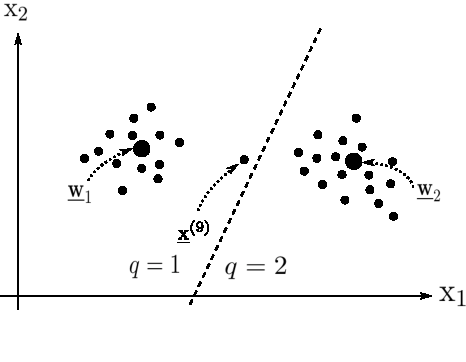
\includegraphics[height=4cm]{img/clustering_soft} 
  \caption{Example for soft clustering. Point (9) is assigned to cluster $1$ with a higher probability than to cluster 2: $\big< m_1^{(9)} \big> = 0.51$, $\big< m_2^{(9)} \big> = 0.49$}
  \label{fig:clusteringsoft}
\end{figure}
\end{frame}

Going back to mean-field approximation:

The approximation is achieved by minimizing the KL-divergence between the distribution $P$ and $Q$. 

\begin{frame}[t] \slidesonly{\frametitle{Minimization of the KL-divergence}}
\begin{block}{Mean Field equation (c.f. section on Stochastic Optimization for how to arrive at this result)}
$$
	\fbox{$ \frac{\partial}{\partial e_l}\big<E_p\big>_Q 
		- \sum\limits_k e_k \frac{\partial}{\partial e_l} \big<s_k\big>_Q = 0
	$}
$$
\end{block}
$$	\frac{\partial \big< E_p \big>_Q}{\partial e_q^{(\alpha)}}
	- \sum\limits_{r, \gamma} \frac{
		\overbrace{ \partial \big< m_r^{(\gamma)} \big>_Q }^{
			\substack{	\text{depends only on} \\
					\text{data point } \gamma }}}{
			\partial e_q^{(\alpha)}}
		e_r^{(\gamma)} \eqexcl 0
$$
$$
	\frac{\partial \big< E_p \big>_Q}{\partial e_q^{(\alpha)}}
	- \sum\limits_r \frac{\partial \big< m_r^{(\alpha)} \big>_Q}{
		\partial e_q^{(\alpha)}}
		e_r^{(\alpha)} \eqexcl 0
$$

switch to lecture slides....
\end{frame}

\mode*

\clearpage

%\section{References}
%\begin{frame}[allowframebreaks] \frametitle{References}
	%\scriptsize
	%\bibliographystyle{plainnat}
	%\bibliography{bibliography}
%\end{frame}

\end{rightcolumn}
\end{paracol}

\end{document}
